\chapter{Datasets}

Dummy text.

\section{Dataset types}

In this section, we introduce the datasets we have used or have considered to use in our work. We divide the datasets in two parts, synthetic and real. Our idea is to use synthetic data to help with training and realize a better prediction on real data.

\subsection{Synthetic data}

For synthetic data we have used SunCG dataset and SIXD toolkit to render some simple views of single object from SunCG .


\subsubsection{SIXD}
\begin{figure}[h!]
  \centering
  \begin{subfigure}[b]{0.32\linewidth}
    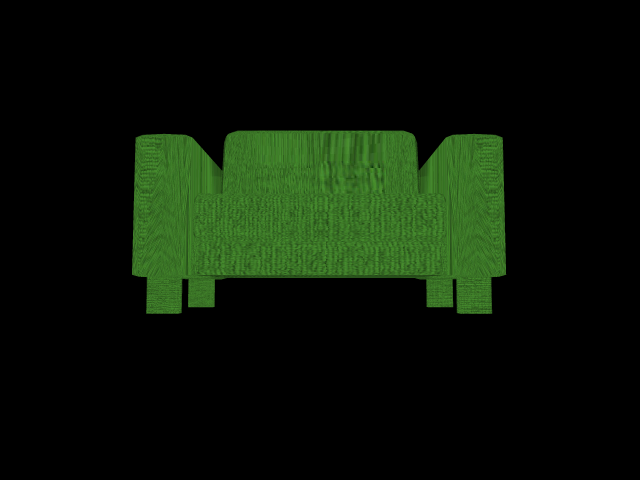
\includegraphics[width=\linewidth]{sixd_sofa_xscale_nobg/0002.png}
  \end{subfigure}
  \begin{subfigure}[b]{0.32\linewidth}
    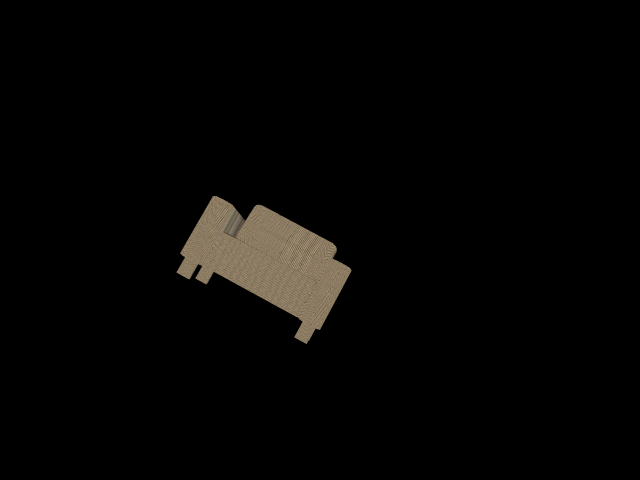
\includegraphics[width=\linewidth]{sixd_sofa_xscale_nobg/0009.png}
  \end{subfigure}
  \begin{subfigure}[b]{0.32\linewidth}
    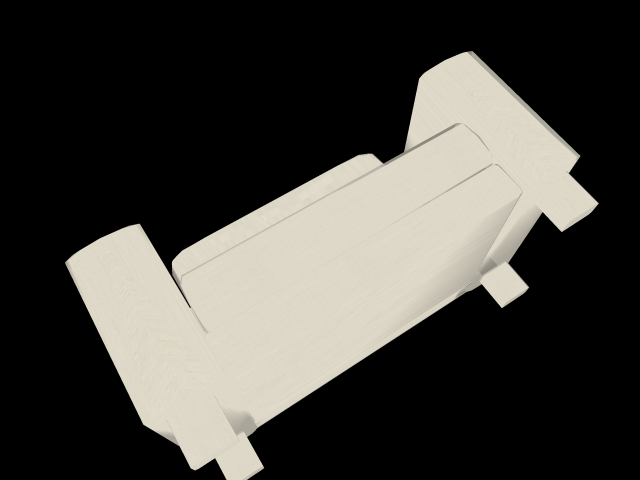
\includegraphics[width=\linewidth]{sixd_sofa_xscale_nobg/0073.png}
  \end{subfigure}
  \begin{subfigure}[b]{0.32\linewidth}
    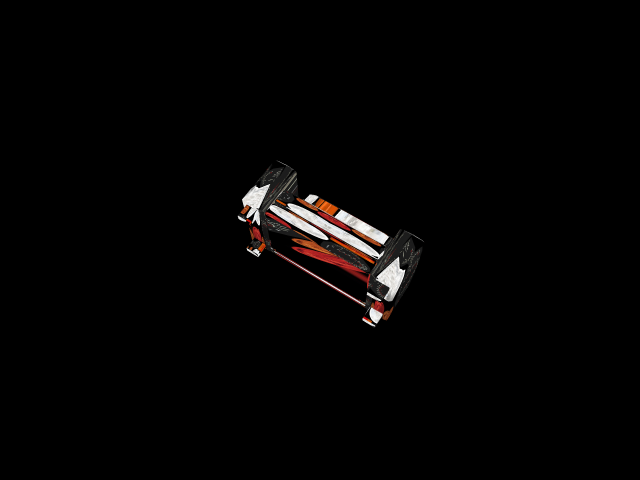
\includegraphics[width=\linewidth]{sixd_sofa_xscale_nobg/0081.png}
  \end{subfigure}
  \begin{subfigure}[b]{0.32\linewidth}
    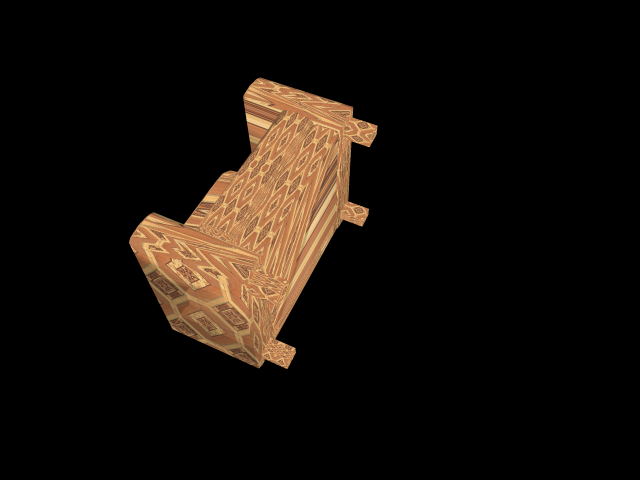
\includegraphics[width=\linewidth]{sixd_sofa_xscale_nobg/0092.png}
  \end{subfigure}
  \begin{subfigure}[b]{0.32\linewidth}
    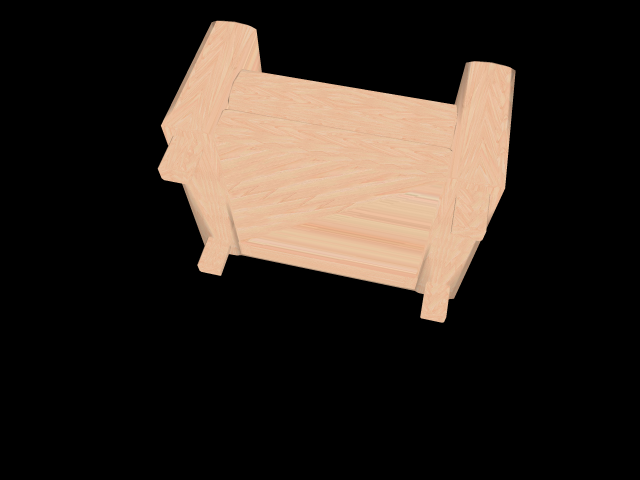
\includegraphics[width=\linewidth]{sixd_sofa_xscale_nobg/0103.png}
  \end{subfigure}
  \begin{subfigure}[b]{0.32\linewidth}
    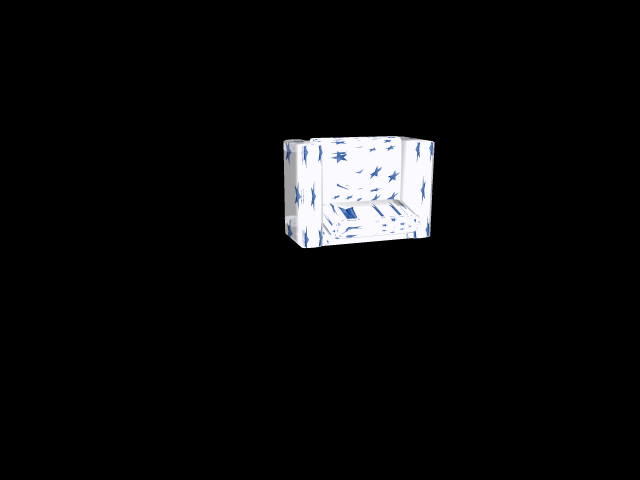
\includegraphics[width=\linewidth]{sixd_sofa_xscale_nobg/0528.png}
  \end{subfigure}
  \begin{subfigure}[b]{0.32\linewidth}
    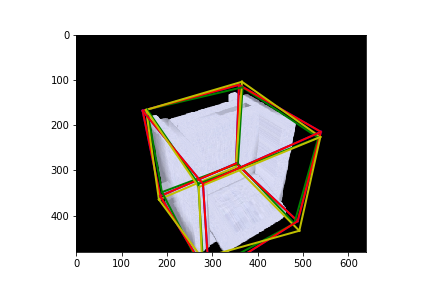
\includegraphics[width=\linewidth]{sixd_sofa_xscale_nobg/0529.png}
  \end{subfigure}
  \begin{subfigure}[b]{0.32\linewidth}
    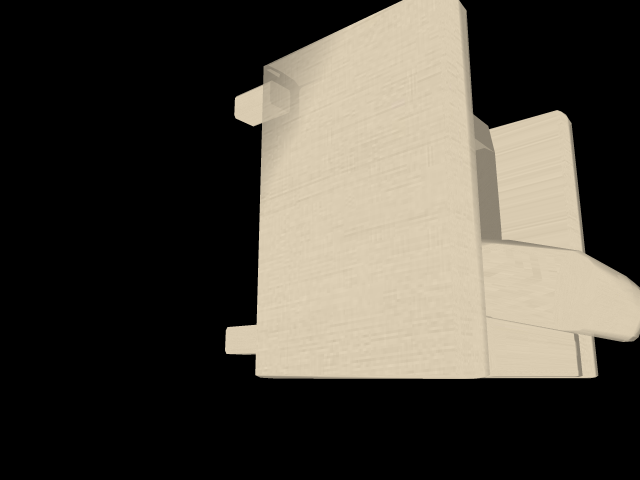
\includegraphics[width=\linewidth]{sixd_sofa_xscale_nobg/0706.png}
  \end{subfigure}
  \begin{subfigure}[b]{0.32\linewidth}
    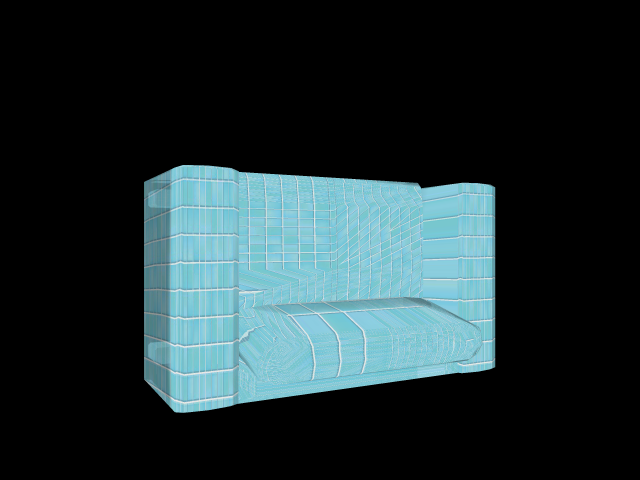
\includegraphics[width=\linewidth]{sixd_sofa_xscale_nobg/0713.png}
  \end{subfigure}
  \begin{subfigure}[b]{0.32\linewidth}
    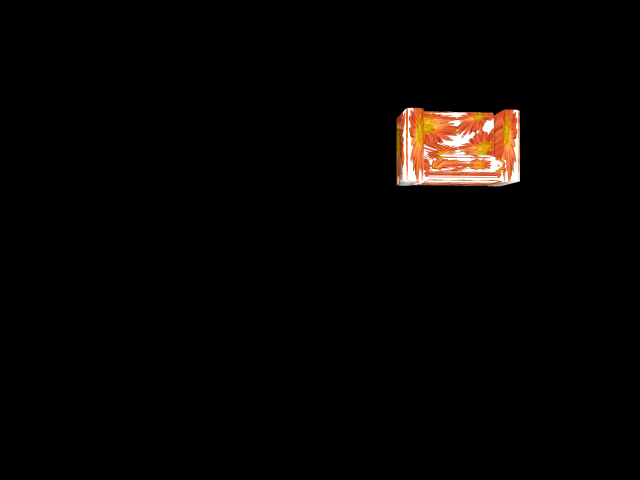
\includegraphics[width=\linewidth]{sixd_sofa_xscale_nobg/0719.png}
  \end{subfigure}
  \begin{subfigure}[b]{0.32\linewidth}
    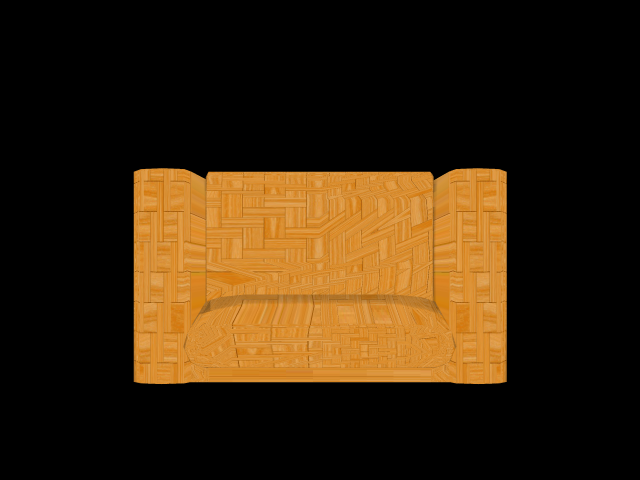
\includegraphics[width=\linewidth]{sixd_sofa_xscale_nobg/0720.png}
  \end{subfigure}
  \begin{subfigure}[b]{0.32\linewidth}
    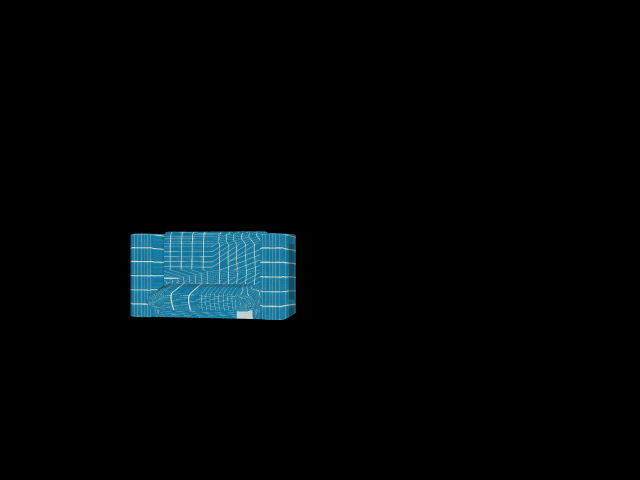
\includegraphics[width=\linewidth]{sixd_sofa_xscale_nobg/0722.png}
  \end{subfigure}
  \begin{subfigure}[b]{0.32\linewidth}
    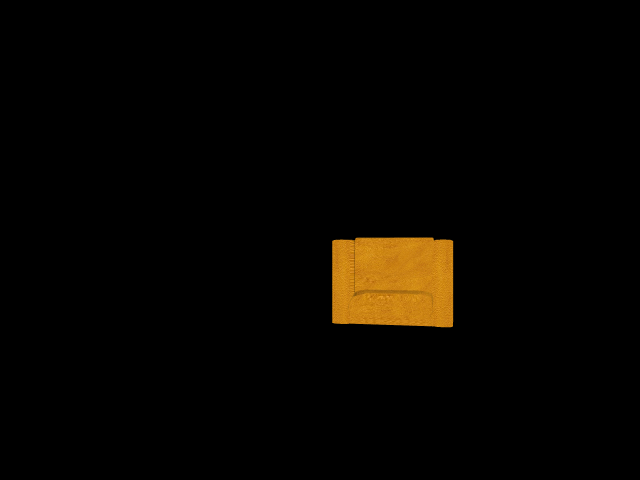
\includegraphics[width=\linewidth]{sixd_sofa_xscale_nobg/0723.png}
  \end{subfigure}
  \begin{subfigure}[b]{0.32\linewidth}
    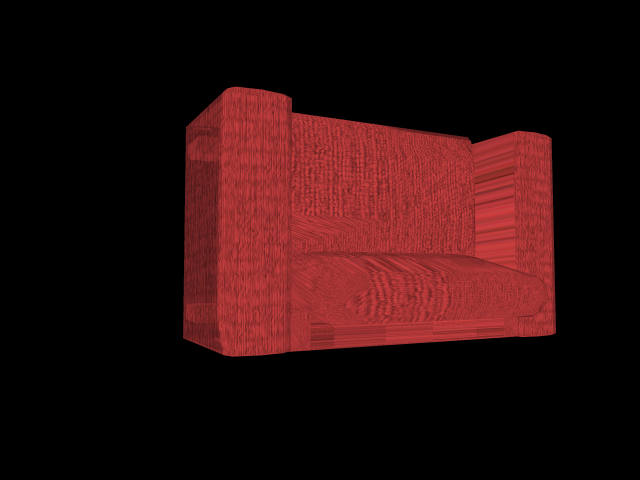
\includegraphics[width=\linewidth]{sixd_sofa_xscale_nobg/0762.png}
  \end{subfigure}
  \begin{subfigure}[b]{0.32\linewidth}
    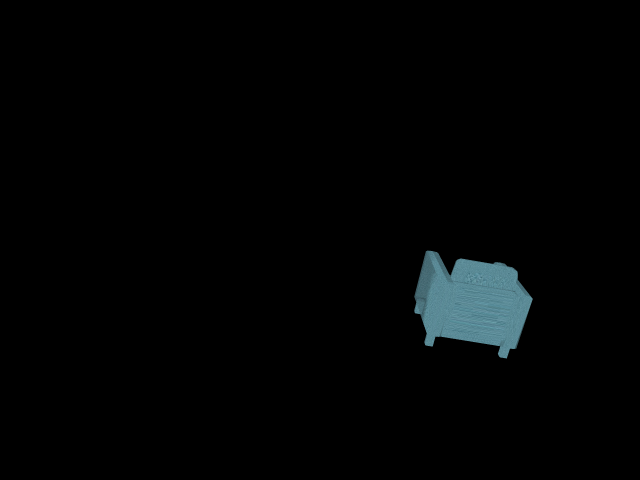
\includegraphics[width=\linewidth]{sixd_sofa_xscale_nobg/1289.png}
  \end{subfigure}
  \begin{subfigure}[b]{0.32\linewidth}
    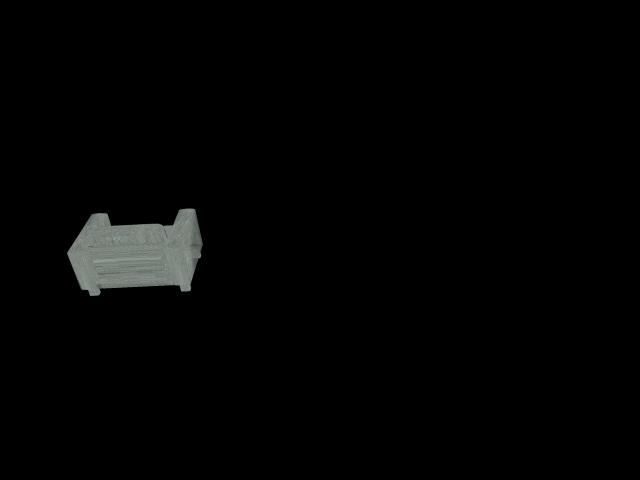
\includegraphics[width=\linewidth]{sixd_sofa_xscale_nobg/1294.png}
  \end{subfigure}
  \begin{subfigure}[b]{0.32\linewidth}
    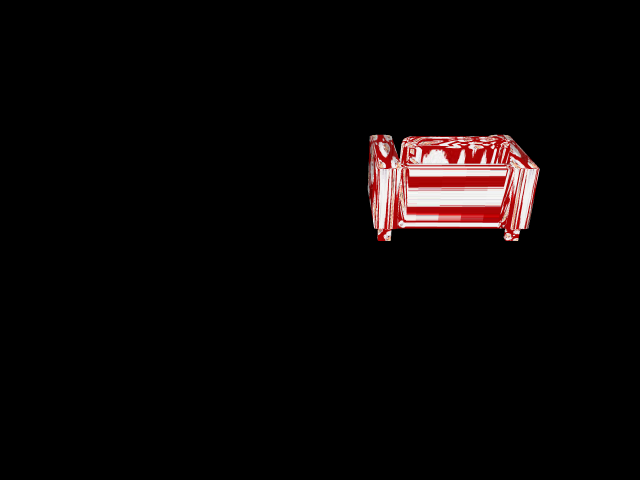
\includegraphics[width=\linewidth]{sixd_sofa_xscale_nobg/1309.png}
  \end{subfigure}
  \caption{SIXD rendering }
  \label{fig:sixd_sofa_xscale_nobg}
\end{figure}

\begin{figure}[h!]
  \centering
  \begin{subfigure}[b]{0.32\linewidth}
    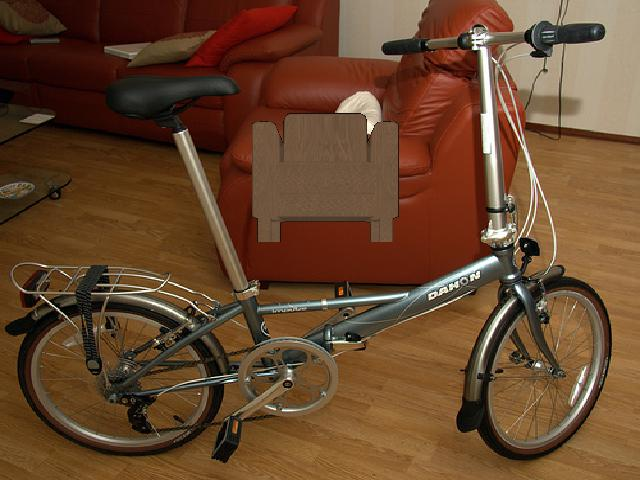
\includegraphics[width=\linewidth]{sixd_sofa_bg/0000.png}
  \end{subfigure}
  \begin{subfigure}[b]{0.32\linewidth}
    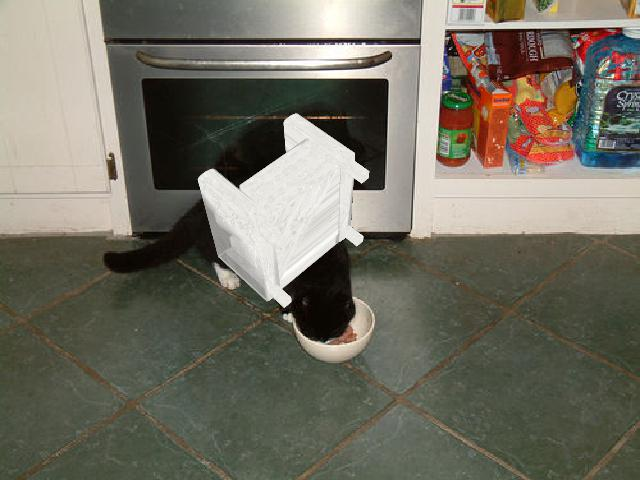
\includegraphics[width=\linewidth]{sixd_sofa_bg/0249.png}
  \end{subfigure}
  \begin{subfigure}[b]{0.32\linewidth}
    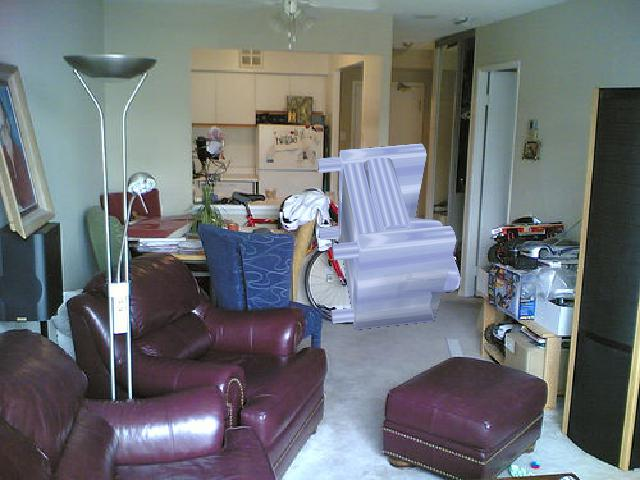
\includegraphics[width=\linewidth]{sixd_sofa_bg/0324.png}
  \end{subfigure}
  \begin{subfigure}[b]{0.32\linewidth}
    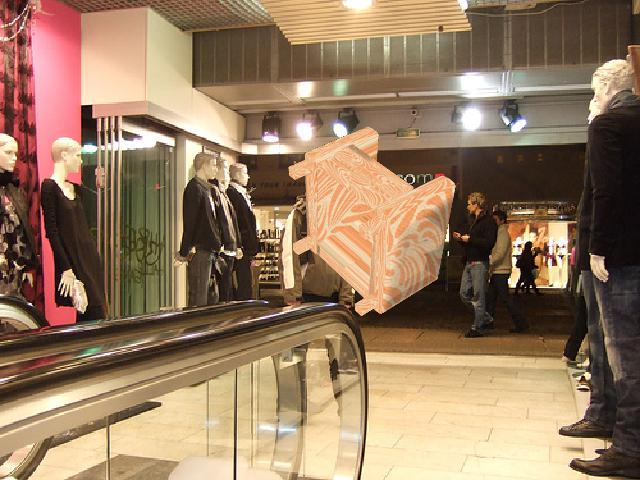
\includegraphics[width=\linewidth]{sixd_sofa_bg/0378.png}
  \end{subfigure}
  \begin{subfigure}[b]{0.32\linewidth}
    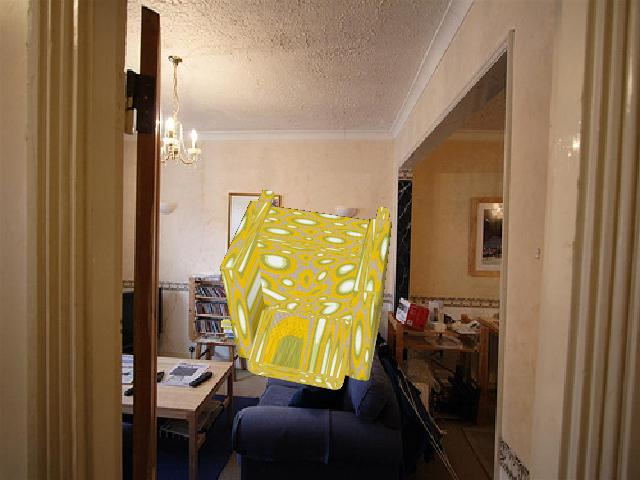
\includegraphics[width=\linewidth]{sixd_sofa_bg/0403.png}
  \end{subfigure}
  \begin{subfigure}[b]{0.32\linewidth}
    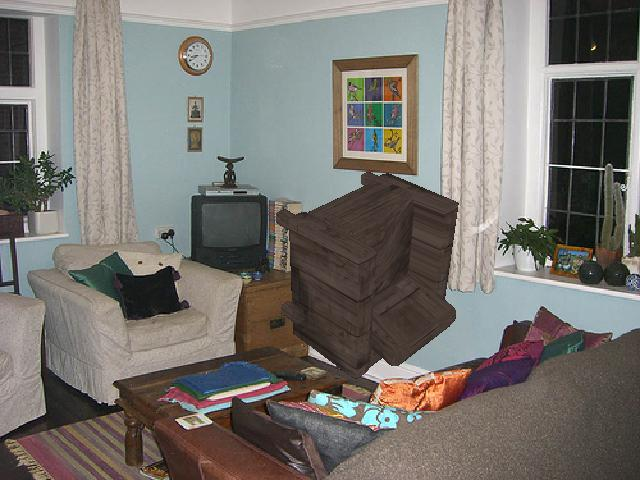
\includegraphics[width=\linewidth]{sixd_sofa_bg/0527.png}
  \end{subfigure}
  \begin{subfigure}[b]{0.32\linewidth}
    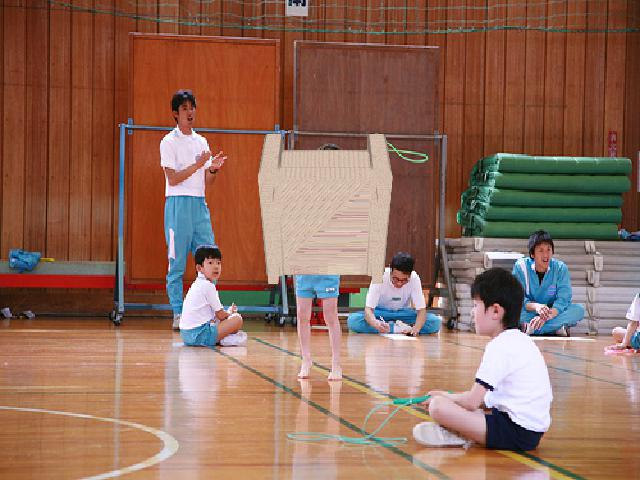
\includegraphics[width=\linewidth]{sixd_sofa_bg/0571.png}
  \end{subfigure}
  \begin{subfigure}[b]{0.32\linewidth}
    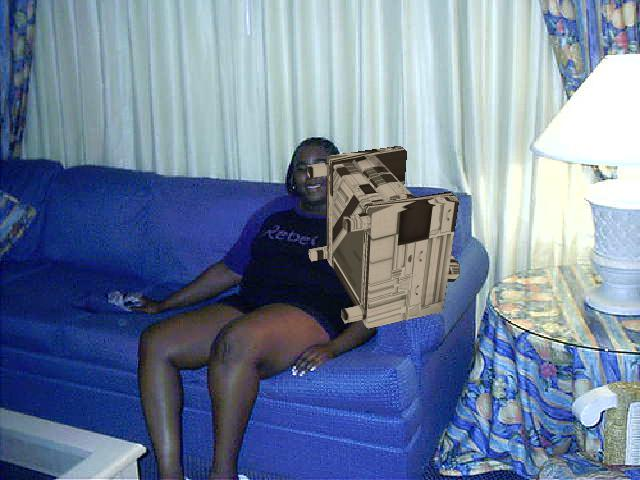
\includegraphics[width=\linewidth]{sixd_sofa_bg/0585.png}
  \end{subfigure}
  \begin{subfigure}[b]{0.32\linewidth}
    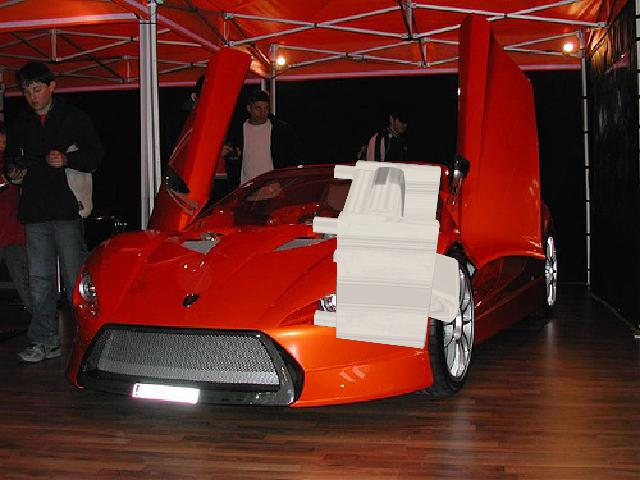
\includegraphics[width=\linewidth]{sixd_sofa_bg/0591.png}
  \end{subfigure}
  \begin{subfigure}[b]{0.32\linewidth}
    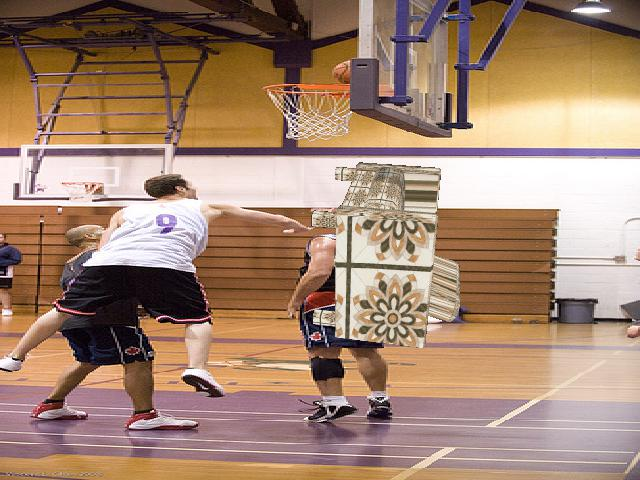
\includegraphics[width=\linewidth]{sixd_sofa_bg/0668.png}
  \end{subfigure}
  \begin{subfigure}[b]{0.32\linewidth}
    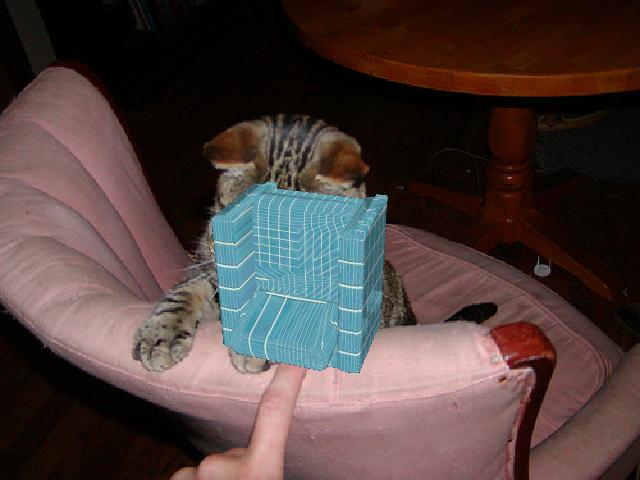
\includegraphics[width=\linewidth]{sixd_sofa_bg/0769.png}
  \end{subfigure}
  \begin{subfigure}[b]{0.32\linewidth}
    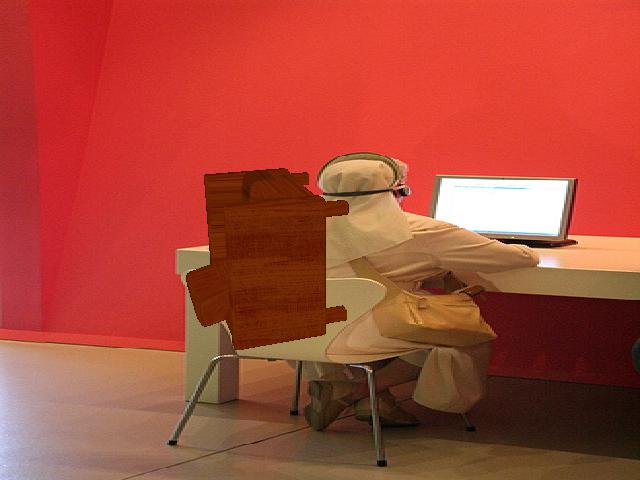
\includegraphics[width=\linewidth]{sixd_sofa_bg/0781.png}
  \end{subfigure}
  \begin{subfigure}[b]{0.32\linewidth}
    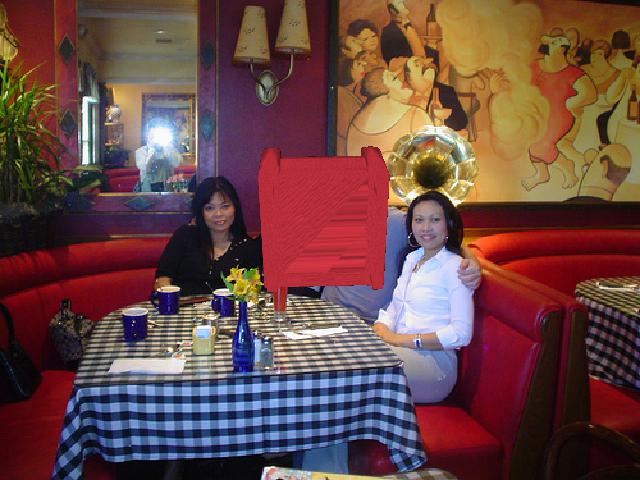
\includegraphics[width=\linewidth]{sixd_sofa_bg/0806.png}
  \end{subfigure}
  \begin{subfigure}[b]{0.32\linewidth}
    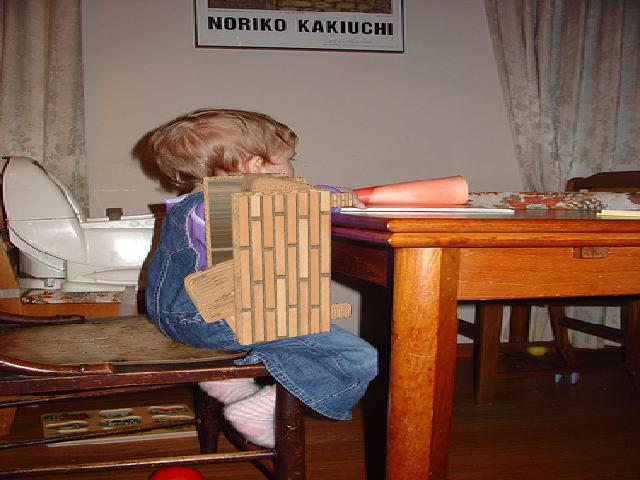
\includegraphics[width=\linewidth]{sixd_sofa_bg/0863.png}
  \end{subfigure}
  \begin{subfigure}[b]{0.32\linewidth}
    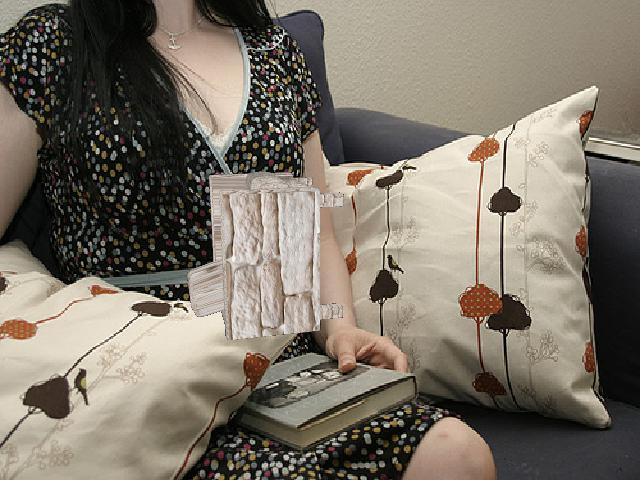
\includegraphics[width=\linewidth]{sixd_sofa_bg/0950.png}
  \end{subfigure}
  \begin{subfigure}[b]{0.32\linewidth}
    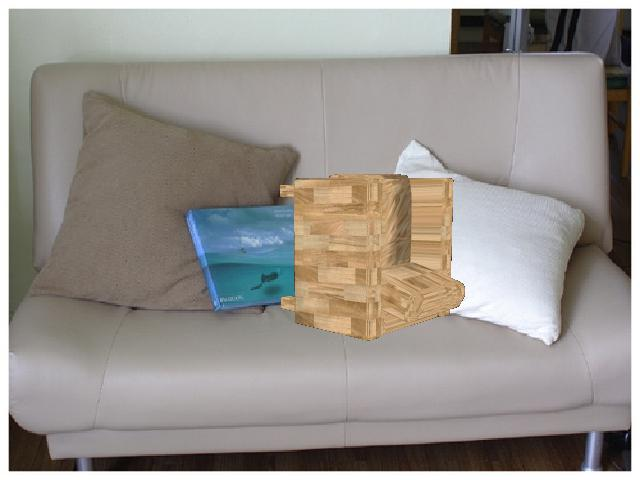
\includegraphics[width=\linewidth]{sixd_sofa_bg/1008.png}
  \end{subfigure}
  \begin{subfigure}[b]{0.32\linewidth}
    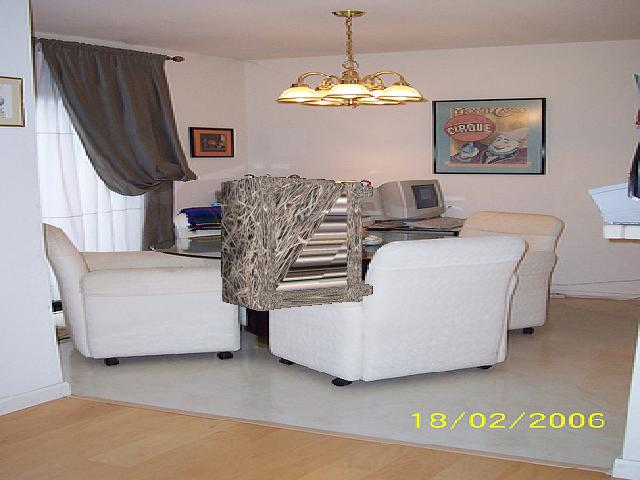
\includegraphics[width=\linewidth]{sixd_sofa_bg/1256.png}
  \end{subfigure}
  \begin{subfigure}[b]{0.32\linewidth}
    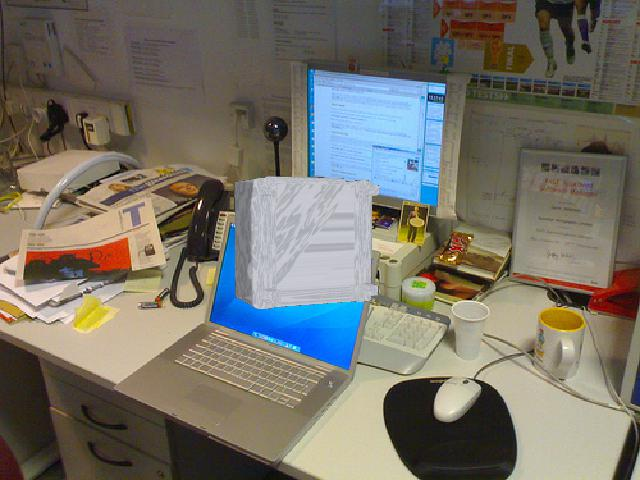
\includegraphics[width=\linewidth]{sixd_sofa_bg/1259.png}
  \end{subfigure}
  \caption{SIXD rendering of sofa in random texture with random background}
  \label{fig:sixd_sofa_bg}
\end{figure}


\subsubsection{SunCG}
SunCG dataset is a manually created large-scale dataset of synthetic 3D scenes with dense volumetric annotations \cite{song2016ssc}
\begin{figure}[h!]
  \centering
  \begin{subfigure}[b]{0.32\linewidth}
    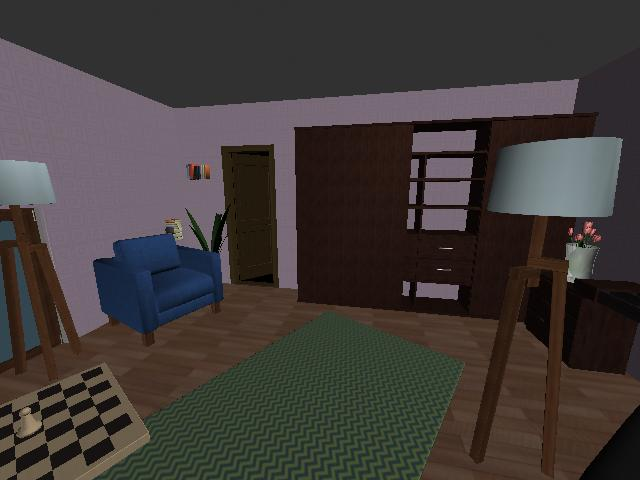
\includegraphics[width=\linewidth]{suncg_dataset/000000_color.jpg}
  \end{subfigure}
  \begin{subfigure}[b]{0.32\linewidth}
    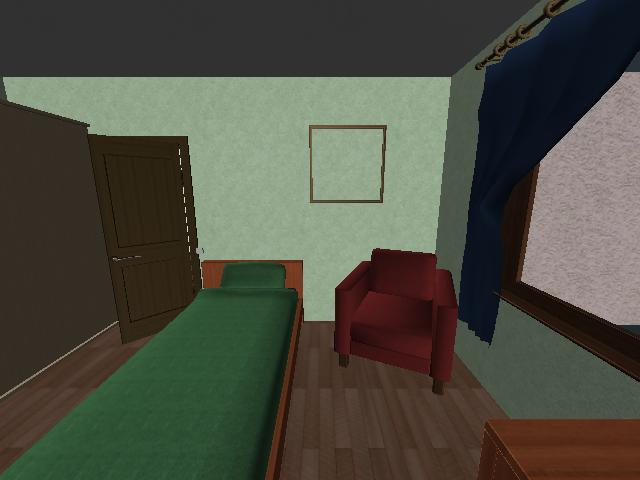
\includegraphics[width=\linewidth]{suncg_dataset/000001_color.jpg}
  \end{subfigure}
  \begin{subfigure}[b]{0.32\linewidth}
    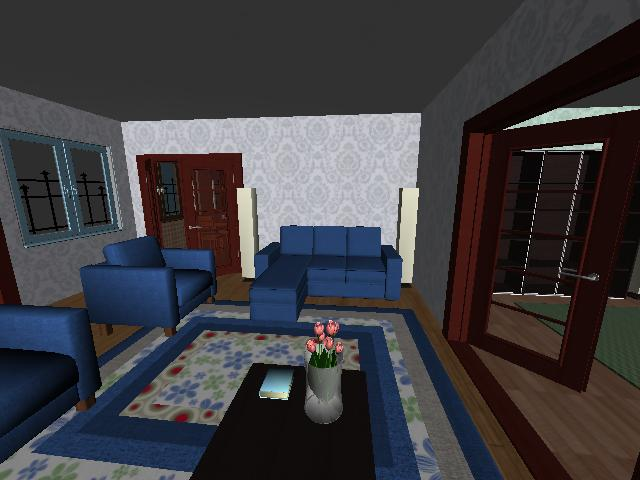
\includegraphics[width=\linewidth]{suncg_dataset/000002_color.jpg}
  \end{subfigure}
  \begin{subfigure}[b]{0.32\linewidth}
    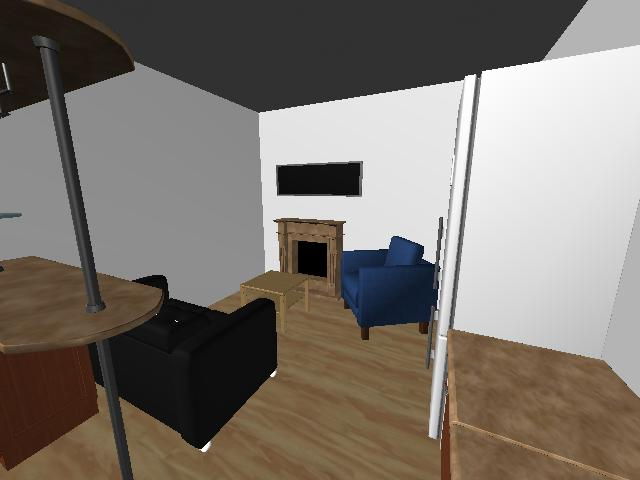
\includegraphics[width=\linewidth]{suncg_dataset/000003_color.jpg}
  \end{subfigure}
  \begin{subfigure}[b]{0.32\linewidth}
    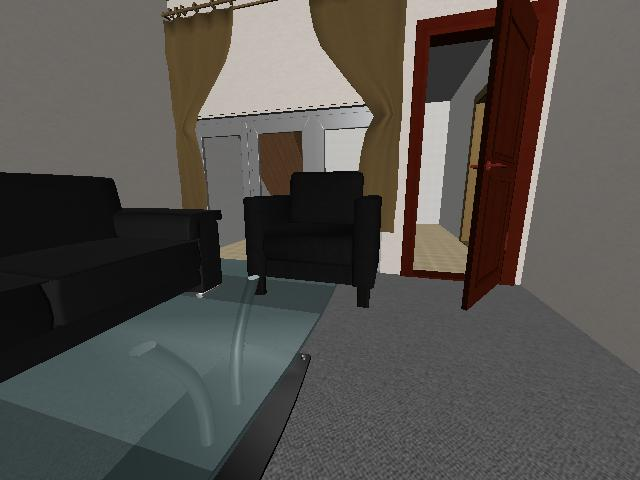
\includegraphics[width=\linewidth]{suncg_dataset/000004_color.jpg}
  \end{subfigure}
  \begin{subfigure}[b]{0.32\linewidth}
    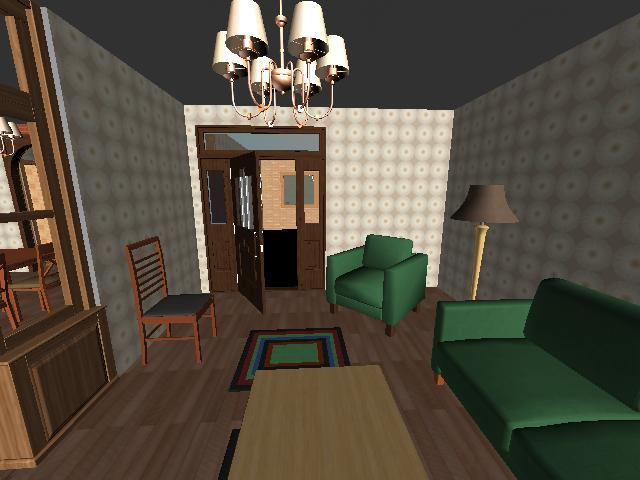
\includegraphics[width=\linewidth]{suncg_dataset/000005_color.jpg}
  \end{subfigure}
  \begin{subfigure}[b]{0.32\linewidth}
    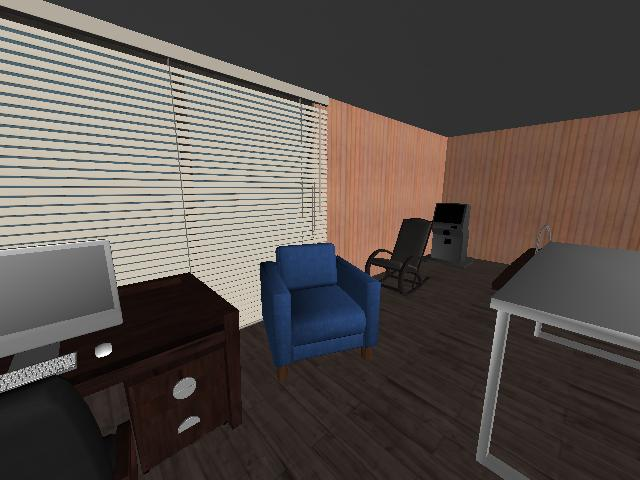
\includegraphics[width=\linewidth]{suncg_dataset/000008_color.jpg}
  \end{subfigure}
  \begin{subfigure}[b]{0.32\linewidth}
    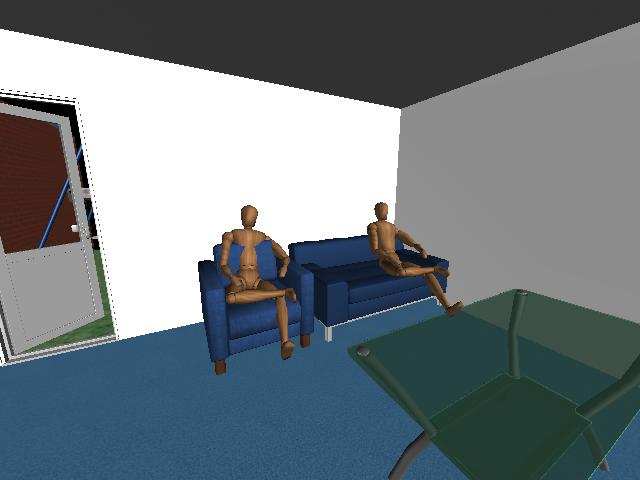
\includegraphics[width=\linewidth]{suncg_dataset/000016_color.jpg}
  \end{subfigure}
  \begin{subfigure}[b]{0.32\linewidth}
    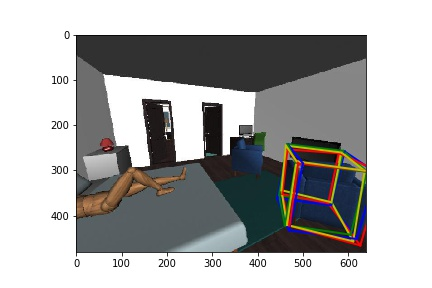
\includegraphics[width=\linewidth]{suncg_dataset/000020_color.jpg}
  \end{subfigure}
  \begin{subfigure}[b]{0.32\linewidth}
    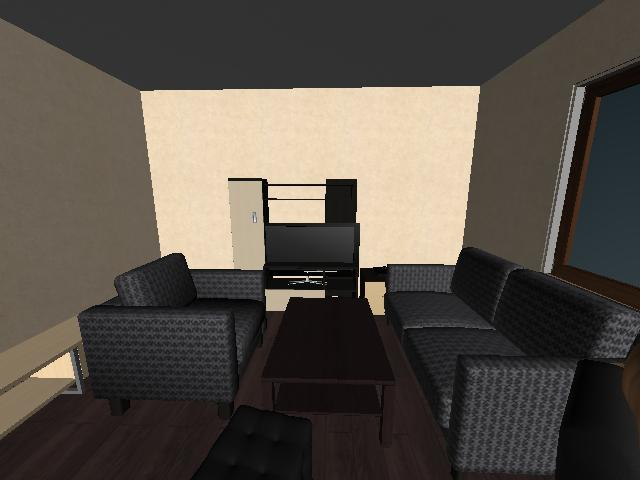
\includegraphics[width=\linewidth]{suncg_dataset/000022_color.jpg}
  \end{subfigure}
  \begin{subfigure}[b]{0.32\linewidth}
    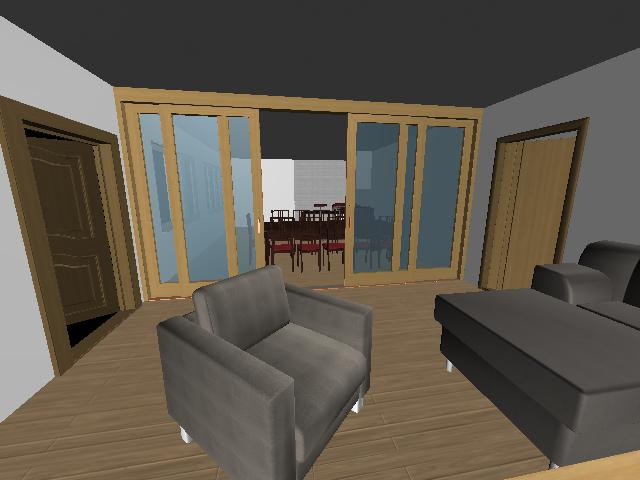
\includegraphics[width=\linewidth]{suncg_dataset/000028_color.jpg}
  \end{subfigure}
  \begin{subfigure}[b]{0.32\linewidth}
    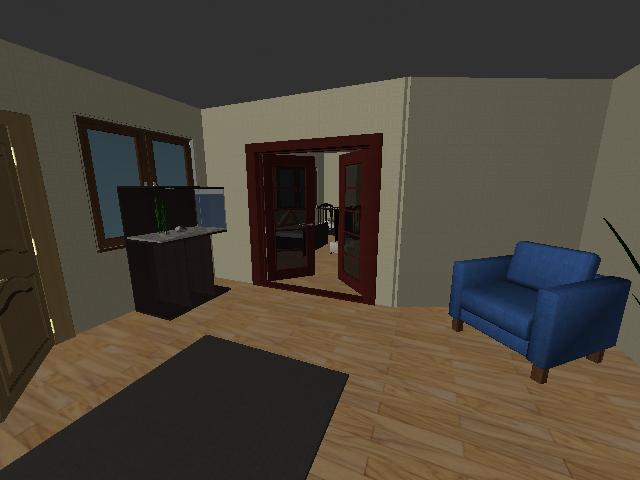
\includegraphics[width=\linewidth]{suncg_dataset/000029_color.jpg}
  \end{subfigure}
  \begin{subfigure}[b]{0.32\linewidth}
    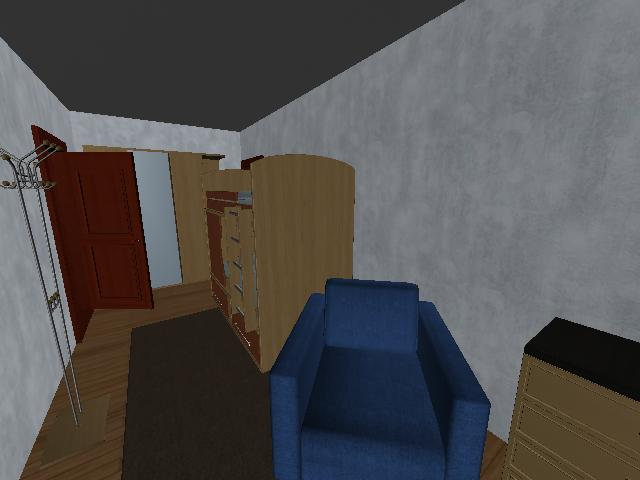
\includegraphics[width=\linewidth]{suncg_dataset/000031_color.jpg}
  \end{subfigure}
  \begin{subfigure}[b]{0.32\linewidth}
    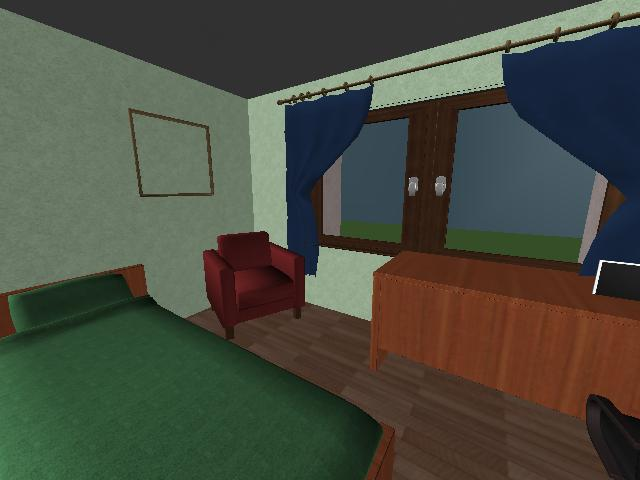
\includegraphics[width=\linewidth]{suncg_dataset/000032_color.jpg}
  \end{subfigure}
  \begin{subfigure}[b]{0.32\linewidth}
    \includegraphics[width=\linewidth]{suncg_dataset/000040_color.jpg}
  \end{subfigure}
  \begin{subfigure}[b]{0.32\linewidth}
    \includegraphics[width=\linewidth]{suncg_dataset/000042_color.jpg}
  \end{subfigure}
  \begin{subfigure}[b]{0.32\linewidth}
    \includegraphics[width=\linewidth]{suncg_dataset/000053_color.jpg}
  \end{subfigure}
  \begin{subfigure}[b]{0.32\linewidth}
    \includegraphics[width=\linewidth]{suncg_dataset/000079_color.jpg}
  \end{subfigure}
  \caption{SunCG of sofa in random texture with random background}
  \label{fig:suncg_dataset}
\end{figure}


\subsection{Real data}
We aim to have a nice generalization of our model to real data. Thus, we mainly focus on the prediction result of our model on datasets consisting real data. In this subsection, we introduce some current datasets containing real data of indoor environments, and elaborate whether they are capable to be used in our work.

\subsubsection{NYU-Depth}
The NYU-Depth V2 dataset is introduced by Silberman et al and originally generated for image segmentation \cite{Silberman:ECCV12}. It is comprised of video sequences from a variety of indoor scenes as recorded by both the RGB and Depth cameras from the Microsoft Kinect. It features 1449 densely labeled pairs of aligned RGB and depth images among 464 scenes taken from 3 cities plus 407,024 unlabeled frames. Each object in the data is labeled with a class and an instance number.

However, the dataset does not provide camera pose information or camera extrinsic parameters for each image, so there is no ground truth for camera location. It also doesn't provide any reconstructed 3D scenes or models, so that we cannot generate ground truth of the 2D coordinates labels for the corresponding 3D keypoints. Thus, NYU-Depth dataset is not applicable for our training or testing procedure.

\subsubsection{7-Scenes}
The 7-Scenes dataset provided by Microsoft Research is a collection of tracked RGB-D camera frames recorded from a handheld Kinect at $640 \times 480$ resolution. It uses KinectFusion system to obtain the ground truth camera tracks and a dense 3D model. Many works and applications in relocalization \cite{shotton2013scene, glocker2013real, wu2017delving} and dense tracking and mapping use 7-scenes for evaluation. While 7-Scenes are available for end-to-end camera pose learning methods, it does not suit for our object pose detection based method.

For the training procedure and labeling, our method needs the object's 3D model and position with respect to the camera as a prior knowledge. 7-Scenes has provided the dense reconstruction represented by signed distance volume of each scene. However, there is no category or object instance labeling related with the 3D scenes. Thus, we cannot get the 3D model and corresponding 2D labels for each object and train for 6D object pose detection. Also, there are limited number of scenes, 7 exactly, which is not enough for our training procedure, where we aim to generalize to as many as possible different scenes. 

During testing, we do not need the 3D object model any more for 6D object pose detection as long as there is trained category object exists in the image. However, our estimation of camera location is with respect to the object. If we have knowledge of the object 3D position with respect to the scene, we can also calculate the camera pose with respect to the scene. 7-Scenes only provides ground truth camera pose with respect to the scene, but do not have any knowledge of the object position. Thus, we cannot compute the camera location with respect to the scenes and 7-Scenes dataset is not applicable for evaluation in our method.

\subsubsection{ScanNet}
ScanNet is originally introduced by Dai et al in 2017 for 3D reconstructions of indoor scenes \cite{dai2017scannet}. ScanNet is an RGB-D video dataset containing 2.5 million views in more than 1500 scans, annotated with 3D camera poses, surface reconstructions, and instance-level semantic segmentations. To collect the data, an easy-to-use and scalable RGB-D capture system includes automated surface reconstruction and crowdsourced semantic annotation is designed. Using this data helps achieve state-of-the-art performance on several 3D scene understanding tasks, including 3D object classification, semantic voxel labeling, and CAD model retrieval.

The instance-level semantic segmentation on the 3D reconstructions helps us to generate our labels in this work. We can use the segmentation information to extract each object and find the tight 3D bounding box of it. Since the object is already in its location with respect to the scene, we can directly use the camera pose provided correspondence to each RGB-image to compute the 2D projections of the 9 control points of the 3D model. However, if we want to compute the camera pose with respect to the scene, we need to save the object position in the scene, and apply the reverse of it after we get the camera pose with respect to the object from PnP algorithm. During evaluation, we would need a 3D model of the object or the locations of the bounding box of the 3D model to compute the camera pose with respect to the object using PnP algorithm. If the object position with respect to the scene is given or saved, we can also compute the camera extrinsic parameters and compare with the ground truth camera pose. Thus, ScanNet is good for both training and testing procedure in our work, and we can use it alone for our training procedure or mix it with SUNCG or sixd rendering images. We use it  as our main testing dataset and aim to realize a good camera localization on this real data of indoor environments.

However, during implementation there are some limitations due to the drawbacks of ScanNet dataset. The error of our labeling is mainly due to the incomplete reconstruction of the 3D models. Firstly, the bounding box of the 3D model is incorrect due to partly reconstruction of some objects. Some of the bounding boxes may turn out to pass through the object instead of bound it. As shown in figure ?, the legs of the chair is not fully constructed in its 3D mesh, and the result labeling shows an error bounding box. This incomplete reconstruction usually happens to the thin or tiny part of the object, due to the noises from scanning. Also, the incompleteness may frequently occur to the back and downside of the object or the side of the object against the wall or facing the floor. Those sides are not well scanned due to hard access of the camera, so they are often poorly reconstructed. Secondly, the bounding box is not well aligned with the axis. Since this dataset is from real data, there is no existing object model as the synthetic dataset provides. We extract the 3D model of the object from the 3D reconstruction of the whole scene using the instance-level segmentation information provided by ScanNet. Thus, our extracted 3D model may not be aligned with the axis. Since our 3D bounding box is calculated by the minimum and maximum values of each axis, we need to rotate the 3D object model to be aligned with the axis to get the tightest bounding box. Since all of the reconstructed object has a upright direction of z = 1, this makes our job easier. We only need to find out the direction in xy plane for aligning the object. In the ideal case, our initial idea is to use PCA to get the axis directions. However, due to the error and noises introduced by reconstruction, the object may not be symmetrically reconstructed. Sometimes one leg of the four legs of the table is missing, leading the PCA direction to be the diagonal of the top of table rectangle. Even though the object is completely reconstructed, the number of points are not equally distributed on the object mesh - one side may have mesh denser vertices than the other side. This also leads to the PCA not aligned with the ideal direction. To address this problem, we rotate the model in xy plane from -30 degree to 30 degree and calculate the new bounding box per 5 degree gap and take the smallest bounding box we ever get. This solves the problem to a large extent, but not very accurate since we set the granularity to 5 degree in trade off with the processing speed. Thirdly, some reconstruction has a distortion. As we can see from figure , the floor of the whole scene is not flat. Thus, the object model is not accurately aligned with z axis sometimes. We can also do the same trick to rotate the object in zx and yz plane, and get the tightest bounding box, but the result is not always better. The main reason is due to incomplete reconstruction as well. As we can see in figure , the most frequently incomplete reconstruction occurs at the bottom back side of the object. When we rotate the couch in yz plane (we assume the longest side is aligned to x axis), the tightest bounding box becomes the one passing though the actual object but bound to the incomplete mesh. Thus, in either way, whether we refine the upright direction or not, we cannot get an ideal result due to the noises introduced by the scanning and reconstruction. Lastly, there is some noise on camera calibration and camera pose. Camera calibration is not very stable for all the scans - each scan may have a bit deviation on camera intrinsic parameters. However, in training and testing time we do not change camera intrinsic parameter depending on the scan that the input image belongs to. Therefore, some noises may be generated from this small error.
 
\subsection{Dataset processing}

In this subsection, we elaborate some aspects we need to note during generating labels and filtering out training and testing data.

\paragraph{Order of corners}
Since our network is to predict the 2D projections of the object's 3D control points, the order of the points is important to be consistent in order not to confuse the network. When we mix the training dataset from ScanNet and SunCG, consistent order of control points between different dataset on the same class object is also necessary. Since in ScanNet the object model is not provided, but we have to extract it from the 3D scene reconstruction according to instance segmentation, we have to find the correct front side of the object in order to generate consistent order of control points. To make sure the front side of the object is facing us, we have to do a PCA on 3D mesh and remember the direction that z axis has greatest value, and then do the PCA agiain on xy plane only for all mesh vertices. The direction of the principal component has to be aligned with our saved direction, otherwise we rotate the 3D mesh 90 degrees or 180 degrees to make the front side consistent over all objects in the same class. In addition, we have to guarantee the rotation matrix constructed by xy plane PCA and z axis satisfying the right hand rule such that z axis component equals 1 in case of any unwanted flipping to the model.

It is also very important that the predicted order of corners is in consistency with the order of our labels. We check the correctness of the ordering as one of our error metrics during testing. For some objects that may not have an obvious front side, for example table in square shape, we may allow a rotation in xy plane for the predicted corners and select the closest to the ground truth corners as the one to calculate loss.

\paragraph{Data filtering}
Our model aims to do camera localization in any indoor environments as long as there is same or similar object in the image as the model has learnt in training procedure. While synthetic dataset can provide exactly same object in different scenes, which may result in a more accurate prediction, real data do not have exactly same object. We hope our model can recognize object in same class with any texture, but we filter out erroneous labels and object that has very different shape with the typical shape of the objects in the class.

Firstly, due to incomplete reconstruction, we may have erroneous labels that passing through the object, or there may be object in very different shape that may increase the difficulty for our network to converge. Thus, we need to filter out those very different 3D models. One reliable method is to compare the 3D meshes in grid granularity, and set a threshold to filter out the low similarity meshes. However, this method may result in big computation offset and also hard to deal with those slight offset cases for a thin plane, for example a table plane in slightly different height may result in very low grid similarity. To generate less computation overhead, we choose to filter out these cases by comparing the size of the bounding box. If the ratio between any side of the length of the bounding box with the bounding box of our chosen object model per class is out of the threshold range, we throw those data away. In this way, it is much easier to compute and is also able to filter out those incomplete reconstruction and those objects in very different shape. Secondly, we also need to filter out those objects that are at the edge of the image. We filter out those images which have center of the object out of the image, and we set that more than 4 among the 8 corners should be within the range of image. Thirdly, we check whether the object is occluded or not in the image. In ScanNet dataset, instance segmentation of each image is provided, and in SunCG, instance labeled images can also be rendered together with the RGB images. Thus, we can check the occlusion simply by comparing the 2D projections of all the vertices in the 3D object mesh with the 2D instance segmentation. We filter out those data that have more than 40\% of vertices occluded in the image. Lastly, there are sometimes invalid camera poses provided or the cases that the 2D projections of the object in the back of the camera, which are also the cases that we have filtered out for our training and testing data.


We provide our codes to automatically generate the labels of all objects and automatically filter out valid training and testing data for future work.



